\documentclass[a4paper]{article}

% --- 从模板引入的宏包和设置 ---
\input{style/ch_xelatex.tex} % 假设这个文件存在并设置了中文环境,若无则需手动设置xeCJK
% \input{style/scala.tex} % 多线程报告中未使用scala,故注释

%代码段设置 (采用模板的设置,但源报告有自己的lstset,如果需要精确匹配源报告代码风格,可以调整)
\lstset{numbers=left,
	basicstyle=\tiny, % 源报告用的是 \ttfamily\footnotesize
	numberstyle=\tiny,
	keywordstyle=\color{blue!70}, % 源报告用 \color{blue}
	commentstyle=\color{red!50!green!50!blue!50}, % 源报告用 \color{green!60!black}
	frame=single, rulesepcolor=\color{red!20!green!20!blue!20},
	escapeinside=``, % 源报告用 {\%*}{*)}
	language=C++, % 从源报告添加
	showstringspaces=false, % 从源报告添加
	breaklines=true, % 从源报告添加
	captionpos=b % 从源报告添加
}

\graphicspath{ {images/} } % 假设图片路径
\usepackage{ctex} % 模板使用ctex,源报告使用xeCJK。ch_xelatex.tex可能处理了
\usepackage{graphicx}

\definecolor{tableheader}{RGB}{13,17,23}
\definecolor{tablebody1}{RGB}{25,29,35}
\definecolor{tablebody2}{RGB}{35,39,45}
\definecolor{textcolor}{RGB}{240,246,252}

\usepackage{color,framed}
\usepackage{listings}
\usepackage{caption} % 源报告也用了
\usepackage{amssymb} % 源报告也用了 (amsmath, amssymb)
\usepackage{amsmath} % 从源报告添加
\usepackage{enumerate}

\usepackage{colortbl}
\usepackage{xcolor} % 源报告也用了
\usepackage{bm}
\usepackage{lastpage}
\usepackage{fancyhdr}
\usepackage{tabularx}
\usepackage{geometry} % 源报告也用了
% \usepackage{minted} % 源报告未使用,且listings已配置
\usepackage{graphics} % graphicx 更常用
\usepackage{subfigure} % 源报告用 subcaption
\usepackage{subcaption} % 从源报告添加
\usepackage{float} % 源报告也用了
% \usepackage{pdfpages} % 源报告未使用
\usepackage{pgfplots} % 源报告未使用
\pgfplotsset{width=10cm,compat=1.9} % 源报告未使用
\usepackage{multirow}
\usepackage{footnote}
\usepackage{booktabs} % 源报告也用了
% \usepackage{verbatimbox} % 源报告未使用
\usepackage{hyperref} % 从源报告添加
\hypersetup{
	colorlinks=true,
	linkcolor=blue,
	filecolor=magenta,      
	urlcolor=cyan,
}
\usepackage{array} % 从源报告添加
\usepackage{siunitx} % 用于统一数字和单位格式
\usepackage{longtable}
\usepackage{siunitx}
\usepackage{makecell} % 用于表头换行
%-----------------------伪代码 (采用模板的 algorithm2e)------------------
\usepackage[linesnumbered,ruled,vlined]{algorithm2e}
\SetKwInput{KwIn}{输入} % 适应中文,源报告用 \algorithmicrequire
\SetKwInput{KwOut}{输出} % 适应中文,源报告用 \algorithmicensure
\SetKwComment{Comment}{// }{}
\SetKwProg{ParFor}{parallel for}{ do}{end for} % 用于表示并行for循环
\SetKw{Spawn}{spawn}
\SetKw{Join}{join}

% \floatname{algorithm}{Algorithm} % algorithm2e 默认是 Algorithm
% \renewcommand{\algorithmicrequire}{\textbf{Input:}} % algorithm2e 使用 \KwIn
% \renewcommand{\algorithmicensure}{\textbf{Output:}} % algorithm2e 使用 \KwOut
% \usepackage{lipsum} % 示例内容,不需要

% --- 以下 breakablealgorithm 定义来自模板,如果算法不跨页可以不用 ---
\makeatletter
\newenvironment{breakablealgorithm}
{% \begin{breakablealgorithm}
		\begin{center}
			\refstepcounter{algorithm}% New algorithm
			\hrule height.8pt depth0pt \kern2pt% \@fs@pre for \@fs@ruled
			\renewcommand{\caption}[2][\relax]{% Make a new \caption
				{\raggedright\textbf{\ALG@name~\thealgorithm} ##2\par}%
				\ifx\relax##1\relax % #1 is \relax
				\addcontentsline{loa}{algorithm}{\protect\numberline{\thealgorithm}##2}%
				\else % #1 is not \relax
				\addcontentsline{loa}{algorithm}{\protect\numberline{\thealgorithm}##1}%
				\fi
				\kern2pt\hrule\kern2pt
			}
		}{% \end{breakablealgorithm}
		\kern2pt\hrule\relax% \@fs@post for \@fs@ruled
	\end{center}
}
\makeatother
%------------------------代码 (listings 设置在上面已经修改)-------------------

%-------------------------页面边距 (采用模板的)--------------
\geometry{a4paper,left=2.3cm,right=2.3cm,top=2.7cm,bottom=2.7cm} %源报告是 margin=1in

%-------------------------页眉页脚 (采用模板的)--------------
\pagestyle{fancy}
\lhead{\kaishu \leftmark}
\rhead{\kaishu 并行程序设计实验报告}%
\lfoot{}
\cfoot{\thepage} % 模板是 \thepage\ of \pageref{LastPage},源报告是 \thepage
\rfoot{}
\renewcommand{\headrulewidth}{0.1pt}
\renewcommand{\footrulewidth}{0pt}
\newcommand{\HRule}{\rule{\linewidth}{0.5mm}}
\newcommand{\HRulegrossa}{\rule{\linewidth}{1.2mm}}
% \setlength{\textfloatsep}{10mm} % 可以按需调整

% --- 针对源报告中 xeCJK 的字体设置,ch_xelatex.tex 可能已处理 ---
% \setCJKmainfont{SimSun} % 设置中文字体,例如宋体
% \setmainfont{Times New Roman} % 设置英文字体

%--------------------文档内容--------------------


\renewcommand{\theadfont}{\bfseries\small} % 定义 \thead 字体为粗体和小号
\sisetup{
	detect-all, % 检测字体设置
	round-mode=places, % round-precision 指定小数位数
	scientific-notation = true, % 强制科学计数法
	exponent-product = \cdot % 使用点作为科学计数法的乘号 (可选)
}
\begin{document}
	\renewcommand{\contentsname}{目\ 录}
	\renewcommand{\appendixname}{附录}
	\renewcommand{\appendixpagename}{附录}
	\renewcommand{\refname}{参考文献} 
	\renewcommand{\figurename}{图}
	\renewcommand{\tablename}{表}
	\renewcommand{\today}{\number\year 年 \number\month 月 \number\day 日}
	
	%-------------------------封面 (采用模板样式,修改内容)----------------
	\begin{titlepage}
		\begin{center}
			\includegraphics[width=0.8\textwidth]{NKU.png}\\[1cm] % 假设NKU.png存在
			\vspace{20mm}
			\textbf{\huge\textbf{\kaishu{计算机学院}}}\\[0.5cm] % 模板内容
			\textbf{\huge{\kaishu{并行程序设计实验报告}}}\\[2.3cm] % 模板内容
			\textbf{\Huge\textbf{\kaishu{多线程并行编程}}}\\[2cm] % 修改为多线程
			
			
			\vspace{\fill}
			
			\centering
			\textsc{\LARGE \kaishu{姓名\ :\ 陈翔}}\\[0.5cm] % 修改为源报告作者
			\textsc{\LARGE \kaishu{学号\ :\ 2314035}}\\[0.5cm] % 占位符
			\textsc{\LARGE \kaishu{专业\ :\ 计算机科学与技术}}\\[0.5cm] % 占位符
			
			\vfill
			{\Large \today}
		\end{center}
	\end{titlepage}
	
	\renewcommand {\thefigure}{\thesection{}.\arabic{figure}}
	\renewcommand{\figurename}{图}
	\renewcommand{\contentsname}{目录}  
	\cfoot{\thepage\ of \pageref{LastPage}}
	
	
	% 生成目录
	\clearpage
	\tableofcontents
	\newpage
	
	%--------------------------正文开始--------------------------------
	\section{实验目的和选题} % 映射自源报告的 "引言"
	近似最近邻搜索 (Approximate Nearest Neighbor Search, ANNS) 是在高维数据空间中高效查找与查询点最相似数据点的关键技术。随着数据规模的急剧增长,精确的暴力搜索方法在性能上已无法满足需求。因此,各种ANNS算法应运而生,它们通过牺牲一定的查找精度来换取搜索效率的大幅提升。
	本实验报告主要关注两种基于倒排索引思想的ANNS算法:IVF (Inverted File Index) 和 IVFADC (Inverted File Index with Asymmetric Distance Computation, 即IVF与PQ乘积量化的结合)。我们将详细阐述这两种算法的并行化思路,并结合Pthread编程实践,通过伪代码展示其核心并行逻辑。最后,将根据提供的实验运行结果,对算法的性能(召回率、查询延迟、构建时间)进行分析。
	
	\section{实验环境} % 映射自源报告的 "实验环境与数据集" (照搬)
	\begin{itemize}
		\item \textbf{数据集}: DEEP100K。
		\begin{itemize}
			\item 基向量 (Base vectors): 100,000 个,维度为 96。
			\item 查询向量 (Query vectors): 10,000 个,维度为 96。
			\item Ground truth: 每个查询提供前100个真实最近邻。
		\end{itemize}
		\item \textbf{并行技术}: Pthreads 用于实现IVF和IVFADC算法内部的并行化,为IVF和IVFADC的索引构建和搜索过程配置了8个Pthread线程。
		\item \textbf{测试规模}: 对2000条查询进行测试,搜索最近的 $k=10$ 个邻居。
		\item \textbf{核心硬件参数(示例)}: 实验通常在多核CPU上运行,例如配置8个Pthreads线程。
		\item \textbf{距离度量}: 实验中,IVF的聚类和粗搜索阶段、PQ的训练和ADC阶段主要使用L2距离(欧氏距离平方),而最终的精确重排阶段和一些基准精确搜索(如Flat Search, SIMD Search)使用内积距离(1 - 内积)。
	\end{itemize}
	
	此外,本次实验的设备条件如下,应实验要求,本次实验在arm架构的服务器下进行,操作系统为Linux系统,具体参数如下:
	\begin{verbatim}
		Architecture:          aarch64
		CPU op-mode(s):        64-bit
		Byte Order:            Little Endian
		Vendor ID:             HiSilicon
		Model name:            Kunpeng-920
		Thread(s) per core:    1
		Core(s) per cluster:   8
		Cluster(s):            1
		NUMA node(s):          1
		memory:                10 GiB
	\end{verbatim}
	
	由于本人进行了perf测试,在华为给出的服务器上不方便进行测试,故采用阿里云的服务器进行测试,具体参数如下:
	\begin{verbatim}
		Architecture:          aarch64  
		CPU op-mode(s):        32-bit, 64-bit  
		Byte Order:            Little Endian  
		Vendor ID:             ARM  
		Model name:            Neoverse-N2  
		Thread(s) per core:    1  
		Core(s) per socket:    8  
		Socket(s):             1  
		NUMA node(s):          1  
		memory:                30 GiB  
		
	\end{verbatim}
	\section{实验代码} % 模板固有部分,源报告无此独立章节
	本实验所有代码和性能测试结果均已经存在github仓库中:\url{https://github.com/HcxoAlbus/NKU-parallel-programming/tree/main/lab3_%E5%A4%9A%E7%BA%BF%E7%A8%8B%E7%BC%96%E7%A8%8B/}。 % 修改为更通用的描述
	% 若有公开代码库,可取消注释并填写:
	% 本实验所有代码均已经存在github仓库中:\url{https://github.com/user/repo/tree/main/lab_multithread} 
	
	\section{算法设计} % 映射自源报告的 "算法原理与实现"
	
	\subsection{IVF (Inverted File Index) 算法}
	IVF算法的核心思想是通过聚类将数据集划分为若干个簇,然后为每个簇建立一个倒排列表,存储属于该簇的向量的ID。查询时,首先找到与查询向量最近的几个簇(nprobe个),然后仅在这些簇对应的倒排列表中的向量进行精确距离计算。
	
	\subsubsection{算法思路} % 整合源报告的 "IVF索引构建" 和 "IVF并行搜索" 的思路部分
	\textbf{IVF索引构建思路}:
	\begin{enumerate}
		\item \textbf{质心初始化}: 使用 K-means++ 等方法初始化 $N_c$ 个聚类质心。
		\item \textbf{并行K-means聚类}:
		迭代执行以下步骤直到收敛或达到最大迭代次数:
		\begin{itemize}
			\item \textbf{分配步骤 (并行)}: 将所有基向量分配给最近的质心。此步骤可通过Pthreads并行化,每个线程处理一部分基向量。每个线程计算其分配到的向量与所有当前质心的距离,找到最近的质心,并为更新质心计算局部和(向量坐标之和)与局部计数。
			\item \textbf{更新步骤 (聚合后串行或并行)}: 聚合所有线程的局部和与局部计数,重新计算每个簇的质心(平均值)。若出现空簇,则进行重新初始化。
		\end{itemize}
		\item \textbf{构建倒排列表}: 遍历所有基向量,根据最终的聚类结果,将每个向量的ID添加到其所属质心对应的倒排列表中。
	\end{enumerate}
	\textbf{IVF并行搜索思路}:
	\begin{enumerate}
		\item \textbf{查找最近质心 (并行)}:
		给定查询向量 $q$ 和参数 $nprobe$,计算 $q$ 与所有 $N_c$ 个质心的距离。此步骤可并行化,每个线程计算 $q$ 与一部分质心的距离。
		\item \textbf{选择候选簇}:
		对所有质心按与 $q$ 的距离排序,选择最近的 $nprobe$ 个质心及其对应的簇。
		\item \textbf{并行搜索倒排列表}:
		对于选中的 $nprobe$ 个簇,并行地在其倒排列表中搜索。每个线程可以负责搜索一个或多个倒排列表。对于列表中的每个向量ID,从原始数据中获取该向量,计算其与查询向量 $q$ 的精确距离。每个线程维护一个局部的Top-k结果优先队列。
		\item \textbf{合并结果}:
		合并所有线程的局部Top-k结果,得到最终的全局Top-k结果。
	\end{enumerate}
	
	\subsubsection{伪代码实现} % 映射自源报告的 "IVF核心伪代码"
	
	\begin{algorithm}[H]
		\caption{IVF K-means 并行分配与质心更新 (单次迭代)}
		\KwIn{基向量集合 $B$, 当前质心 $C_{old}$, 线程数 $T$}
		\KwOut{新质心 $C_{new}$, 向量分配 $Assignments$}
		初始化全局新质心累加和 $GlobalSums[1..N_c]$ 为0, 全局计数 $GlobalCounts[1..N_c]$ 为0\;
		\ParFor{$t = 1$ \KwTo $T$ \Comment*[r]{Pthread工作线程}}{
			初始化线程局部累加和 $LocalSums_t[1..N_c]$ 为0, 局部计数 $LocalCounts_t[1..N_c]$ 为0\;
			\For{每个分配给线程 $t$ 的基向量 $b_i \in B_{subset\_t}$}{
				$min\_dist \leftarrow \infty$\; $best\_cluster \leftarrow -1$\;
				\For{$j = 1$ \KwTo $N_c$}{
					$dist \leftarrow \text{distance}(b_i, C_{old}[j])$\;
					\If{$dist < min\_dist$}{
						$min\_dist \leftarrow dist$\;
						$best\_cluster \leftarrow j$\;
					}
				}
				$Assignments[i] \leftarrow best\_cluster$\;
				$LocalSums_t[best\_cluster] \leftarrow LocalSums_t[best\_cluster] + b_i$\;
				$LocalCounts_t[best\_cluster] \leftarrow LocalCounts_t[best\_cluster] + 1$\;
			}
		}
		\tcc{主线程聚合}
		\For{$j = 1$ \KwTo $N_c$}{
			\For{$t = 1$ \KwTo $T$}{
				$GlobalSums[j] \leftarrow GlobalSums[j] + LocalSums_t[j]$\;
				$GlobalCounts[j] \leftarrow GlobalCounts[j] + LocalCounts_t[j]$\;
			}
			\If{$GlobalCounts[j] > 0$}{
				$C_{new}[j] \leftarrow GlobalSums[j] / GlobalCounts[j]$\;
			}
			\Else{
				$C_{new}[j] \leftarrow \text{reinitialize\_centroid}()$ \Comment*[r]{处理空簇}\;
			}
		}
	\end{algorithm}
	
	\begin{algorithm}[H]
		\caption{IVF 并行搜索}
		\KwIn{查询向量 $q$, IVF索引 $Index$, Top-k参数 $k$, 探查簇数 $nprobe$, 线程数 $T$}
		\KwOut{Top-k结果 $ResultsHeap$}
		$CentroidDists \leftarrow \text{empty list}$\;
		\ParFor{$t = 1$ \KwTo $T$ \Comment*[r]{阶段1: 并行计算与质心距离}}{
			\For{每个分配给线程 $t$ 的质心 $c_j \in Index.centroids_{subset\_t}$}{
				$dist \leftarrow \text{distance}(q, c_j)$\;
				添加 $(dist, j)$ 到线程局部列表 $LocalCentroidDists_t$\;
			}
		}
		\tcc{主线程聚合与选择}
		$AllCentroidDists \leftarrow \text{merge all } LocalCentroidDists_t$\;
		对 $AllCentroidDists$ 按距离排序\;
		$CandidateClusterIndices \leftarrow \text{前 } nprobe \text{ 个簇的索引 from } AllCentroidDists$\;
		
		$GlobalResultsHeap \leftarrow \text{empty max-priority queue of size } k$\;
		\ParFor{$t = 1$ \KwTo $T$ \Comment*[r]{阶段2: 并行搜索倒排列表}}{
			$ThreadResultsHeap_t \leftarrow \text{empty max-priority queue of size } k$\;
			\For{每个分配给线程 $t$ 的簇索引 $cluster\_idx \in CandidateClusterIndices_{subset\_t}$}{
				$InvertedList \leftarrow Index.inverted\_lists[cluster\_idx]$\;
				\For{每个向量ID $vec\_id \in InvertedList$}{
					$base\_vector \leftarrow Index.base\_data[vec\_id]$\;
					$dist \leftarrow \text{distance}(q, base\_vector)$ \Comment*[r]{通常是内积距离}\;
					\If{$ThreadResultsHeap_t.size() < k$}{
						$ThreadResultsHeap_t.push((dist, vec\_id))$\;
					}
					\ElseIf{$dist < ThreadResultsHeap_t.top().first$}{
						$ThreadResultsHeap_t.pop()$\;
						$ThreadResultsHeap_t.push((dist, vec\_id))$\;
					}
				}
			}
		}
		\tcc{主线程合并最终结果}
		\For{$t = 1$ \KwTo $T$}{
			\While{$ThreadResultsHeap_t$ is not empty}{
				$(dist, vec\_id) \leftarrow ThreadResultsHeap_t.pop()$\;
				\If{$GlobalResultsHeap.size() < k$}{
					$GlobalResultsHeap.push((dist, vec\_id))$\;
				}
				\ElseIf{$dist < GlobalResultsHeap.top().first$}{
					$GlobalResultsHeap.pop()$\;
					$GlobalResultsHeap.push((dist, vec\_id))$\;
				}
			}
		}
		$ResultsHeap \leftarrow GlobalResultsHeap$\;
	\end{algorithm}
	
	\subsection{IVFADC (IVF with Product Quantization) 算法}
	IVFADC算法结合了IVF的粗粒度划分和PQ (Product Quantization) 的细粒度压缩,旨在平衡搜索效率、内存占用和召回率。PQ将高维向量切分为若干个子向量,并对每个子空间分别进行量化。IVFADC在IVF的倒排列表中通常存储的是基向量的PQ编码(或其ID,间接指向PQ编码),而不是原始向量,从而大大减少了存储空间和距离计算的开销。
	
	IVF与PQ的结合主要有两种策略:
	\begin{enumerate}
		\item \textbf{方法一 (PQ-then-IVF)}: 先对所有基向量进行PQ编码,然后基于这些编码(或由编码重构出的近似向量)构建IVF索引。
		\item \textbf{方法二 (IVF-then-PQ / 经典IVFADC)}: 先对原始基向量构建IVF索引(确定簇的划分),然后对基向量进行PQ编码,在搜索时利用这些PQ编码进行近似距离计算。
	\end{enumerate}
	下面分别详细介绍这两种方法的思路与实现。
	
	\subsubsection{方法一:先PQ编码(及重构),后构建IVF索引 (PQ-then-IVF)}
	这种方法首先利用乘积量化压缩整个数据集,然后在压缩后的数据(或其重构版本)上建立倒排文件索引。
	
	\paragraph{算法思路}
	\subparagraph{索引构建思路 (PQ-then-IVF)}
	\begin{enumerate}
		\item \textbf{PQ训练与编码}:
		\begin{itemize}
			\item 从基向量中选取训练集(或全部),训练PQ量化器,得到包含 $M \times K_{sub}$ 个码字的码本。
			\item 对数据集中的所有基向量 $b_i$ 进行PQ编码,得到PQ码 $code_i$。
		\end{itemize}
		\item \textbf{数据准备 (用于IVF构建)}:
		\begin{itemize}
			\item \textbf{重构向量}: 使用PQ码本和每个向量的PQ码 $code_i$,重构出近似向量 $b'_i$。得到重构向量集 $B'$。这是常见做法。
			\item (备选:直接使用PQ码,但这要求IVF的距离计算能直接作用于PQ码序列,不常见。)
		\end{itemize}
		\item \textbf{IVF索引构建 (在 $B'$ 上)}:
		\begin{itemize}
			\item \textbf{质心初始化与聚类}: 在重构向量集 $B'$ 上运行K-means算法(例如,使用L2距离),得到 $N_c$ 个IVF聚类质心 $C'_{IVF}$。这些质心本身也是重构向量的形式。
			\item \textbf{分配与构建倒排列表}: 将每个重构向量 $b'_i \in B'$ 分配给其最近的IVF质心 $c'_j \in C'_{IVF}$。在对应质心 $c'_j$ 的倒排列表中,存储原始基向量的ID (即 $b_i$ 的ID)。
		</itemize>
	</end{enumerate}
	
	\subparagraph{并行搜索思路 (PQ-then-IVF)}
	\begin{enumerate}
		\item \textbf{查询向量处理}:
		\begin{itemize}
			\item 给定查询向量 $q$,首先使用训练好的PQ量化器对其进行编码,然后重构得到近似查询向量 $q'$。
		</itemize}
		\item \textbf{查找最近IVF质心 (并行, 基于重构向量)}:
		\begin{itemize}
			\item 并行计算重构查询向量 $q'$ 与所有IVF质心 $C'_{IVF}$ (它们也是重构向量形式) 之间的距离(例如L2距离)。
			\item 选择与 $q'$ 最近的 $nprobe$ 个IVF质心及其对应的簇。
		</itemize}
		\item \textbf{收集候选ID}:
		\begin{itemize}
			\item 从选中的 $nprobe$ 个簇的倒排列表中,收集所有原始基向量的ID。设这些ID构成候选集 $Candidates_{ID}$。
		</itemize}
		\item \textbf{精确重排 (并行)}:
		\begin{itemize}
			\item 对于 $Candidates_{ID}$ 中的每一个原始向量ID:
			\item 从存储中获取原始的高维向量 $b_{orig}$。
			\item 计算原始查询向量 $q$ 与 $b_{orig}$ 之间的精确距离(例如内积距离或精确L2距离)。
			\item 此步骤可并行化,每个线程处理一部分候选ID。每个线程维护一个局部的Top-k结果优先队列。
		</itemize}
		\item \textbf{合并结果}:
		\begin{itemize}
			\item 合并所有线程的局部Top-k结果,得到最终的全局Top-k结果。
		</itemize}
	</end{enumerate}
	
	\begin{algorithm}[H]
		\caption{PQ-then-IVF 索引构建 (方法一)}
		\KwIn{原始基向量 $B_{orig}$, PQ参数 ($M, K_{sub}$), IVF参数 ($N_c, KmeansIter$), 线程数 $T$}
		\KwOut{PQ-IVF索引 $Index_{PQ\_IVF}$ (含PQ量化器, IVF质心(重构形式), 倒排列表(原始ID))}
		
		\tcc{1. PQ部分:训练、编码、重构}
		$PQ\_quantizer \leftarrow \text{new ProductQuantizer}(M, K_{sub})$\;
		$PQ\_quantizer.\text{train}(B_{orig})$ \Comment*[r]{训练PQ码本}
		$B_{codes} \leftarrow PQ\_quantizer.\text{encode}(B_{orig})$ \Comment*[r]{并行编码所有基向量}
		$B_{reco} \leftarrow PQ\_quantizer.\text{reconstruct}(B_{codes})$ \Comment*[r]{并行重构所有基向量}
		
		\tcc{2. IVF部分:在重构数据上构建IVF索引}
		$IVF\_centroids_{reco} \leftarrow \text{KMeans++Init}(B_{reco}, N_c)$\;
		\For{$iter = 1$ \KwTo $KmeansIter$}{
			$(\text{Assignments}_{reco}, \text{Sums}_{reco}, \text{Counts}_{reco}) \leftarrow \text{ParallelKMeansAssign}(B_{reco}, IVF\_centroids_{reco}, T)$\;
			$IVF\_centroids_{reco} \leftarrow \text{UpdateCentroids}(\text{Sums}_{reco}, \text{Counts}_{reco})$\;
			\If{converged}{break\;}
		}
		$InvertedLists_{orig\_ID} \leftarrow \text{empty lists for } N_c \text{ clusters}$\;
		\For{$i = 0$ \KwTo $|B_{orig}|-1$}{
			$reco\_vec \leftarrow B_{reco}[i]$\;
			$cluster\_idx \leftarrow \text{FindNearestCentroid}(reco\_vec, IVF\_centroids_{reco})$\;
			$InvertedLists_{orig\_ID}[cluster\_idx].\text{add}(\text{OriginalID}(B_{orig}[i]))$\;
		}
		$Index_{PQ\_IVF} \leftarrow (PQ\_quantizer, IVF\_centroids_{reco}, InvertedLists_{orig\_ID})$\;
	\end{algorithm}
	
	\begin{algorithm}[H]
		\caption{PQ-then-IVF 并行搜索 (方法一)}
		\KwIn{原始查询 $q_{orig}$, PQ-IVF索引 $Index_{PQ\_IVF}$, Top-k $k$, 探查簇数 $nprobe$, 线程数 $T$, 原始基向量库 $B_{orig\_full}$}
		\KwOut{Top-k结果 $ResultsHeap$}
		
		\tcc{1. 查询向量重构}
		$q_{reco} \leftarrow Index_{PQ\_IVF}.PQ\_quantizer.\text{reconstruct}(Index_{PQ\_IVF}.PQ\_quantizer.\text{encode}(q_{orig}))$\;
		
		\tcc{2. 查找最近IVF质心 (在重构空间)}
		$CentroidDists_{reco} \leftarrow \text{empty list}$\;
		\ParFor{$t = 1$ \KwTo $T$}{
			\For{每个分配给线程 $t$ 的IVF质心 $c'_j \in Index_{PQ\_IVF}.IVF\_centroids_{reco}$}{
				$dist \leftarrow \text{distance}(q_{reco}, c'_j)$ \Comment*[r]{L2距离 on reco}
				添加 $(dist, j)$ 到线程局部列表 $LocalCentroidDists_t$\;
			}
		}
		$AllCentroidDists_{reco} \leftarrow \text{merge all } LocalCentroidDists_t$\;
		对 $AllCentroidDists_{reco}$ 按距离排序\;
		$CandidateClusterIndices \leftarrow \text{前 } nprobe \text{ 个簇的索引 from } AllCentroidDists_{reco}$\;
		
		\tcc{3. 收集候选原始ID并精确重排}
		$GlobalResultsHeap \leftarrow \text{empty max-priority queue of size } k$\;
		\ParFor{$t = 1$ \KwTo $T$}{
			$ThreadResultsHeap_t \leftarrow \text{empty max-priority queue of size } k$\;
			\For{每个分配给线程 $t$ 的簇索引 $cluster\_idx \in CandidateClusterIndices$}{
				$OrigIDsInList \leftarrow Index_{PQ\_IVF}.InvertedLists_{orig\_ID}[cluster\_idx]$\;
				\For{每个原始向量ID $orig\_id \in OrigIDsInList$}{
					$base\_vector_{orig} \leftarrow B_{orig\_full}[orig\_id]$\;
					$dist_{exact} \leftarrow \text{distance\_exact}(q_{orig}, base\_vector_{orig})$\;
					\If{$ThreadResultsHeap_t.size() < k$ \textbf{or} $dist_{exact} < ThreadResultsHeap_t.top().first$}{
						管理 $ThreadResultsHeap_t$ 添加 $(dist_{exact}, orig\_id)$\;
					}
				}
			}
		}
		\tcc{主线程合并最终结果}
		合并所有 $ThreadResultsHeap_t$ 到 $GlobalResultsHeap$\;
		$ResultsHeap \leftarrow GlobalResultsHeap$\;
	\end{algorithm}
	
	\subsubsection{方法二:先构建IVF索引,后利用PQ编码进行距离近似 (经典IVFADC)}
	这是更常见的IVFADC实现方式,先通过IVF对原始数据进行粗粒度划分,然后利用PQ编码进行存储压缩和快速的近似距离计算(ADC)。
	
	\paragraph{算法思路} % 原 4.2.1
	\subparagraph{索引构建思路 (经典IVFADC)} % 原 "IVFADC索引构建思路"
	\begin{enumerate}
		\item \textbf{IVF部分构建 (基于原始数据)}:
		与标准IVF类似,使用K-means(通常基于L2距离)对\textbf{原始}基向量进行聚类,得到 $N_{ivf\_clusters}$ 个IVF质心。然后,将所有基向量分配到相应的IVF簇,并记录它们的原始ID到对应的倒排列表中。
		\item \textbf{PQ部分构建}:
		\begin{itemize}
			\item \textbf{训练PQ量化器}: 从基向量中选取一部分(或全部)作为训练集。将向量维度 $D$ 划分为 $M$ 个子空间,每个子空间的维度为 $D/M$。对每个子空间中的子向量独立进行K-means聚类(例如,每个子空间聚为 $K_{sub}=256$ 个质心,即码字)。所有 $M \times K_{sub}$ 个码字构成了PQ的码本。
			\item \textbf{编码基向量}: 对数据集中的所有基向量,将其每个子向量替换为其在该子空间中最近的码字的ID。因此,每个高维向量被压缩为一个由 $M$ 个ID组成的PQ码。这些PQ码由PQ量化器统一管理。
		</itemize}
		\item \textbf{存储关联}: IVF的倒排列表存储的是原始向量的ID。在搜索时,通过这些ID可以获取到对应向量的PQ编码,用于ADC计算。
	</end{enumerate}
	\subparagraph{并行搜索思路 (经典IVFADC)} % 原 "IVFADC并行搜索思路"
	\begin{enumerate}
		\item \textbf{查找最近IVF质心 (并行, 基于原始查询与原始IVF质心)}:
		与IVF类似,给定查询向量 $q$,并行计算 $q$ 与所有IVF质心的距离(通常用L2距离),选出 $nprobe$ 个最近的IVF簇。
		\item \textbf{预计算查询与PQ码本的距离表 (串行或并行)}:
		对于查询向量 $q$,预先计算其每个子向量与PQ码本中对应子空间所有码字之间的距离,生成一个距离查找表 (Asymmetric Distance Table, ADT)。此表用于快速计算 $q$ 与PQ编码向量的近似距离。
		\item \textbf{并行搜索倒排列表 (使用PQ近似距离)}:
		对于选中的 $nprobe$ 个IVF簇,并行地处理它们的倒排列表。每个线程负责一部分簇。
		\begin{itemize}
			\item 对于倒排列表中的每个向量ID,从PQ量化器获取其PQ编码。
			\item 使用预计算的距离查找表ADT和该向量的PQ编码,计算查询向量 $q$ 与该PQ编码向量之间的近似L2距离 (ADC - Asymmetric Distance Computation)。
			\item 每个线程维护一个局部的Top-$k_{cand}$ 候选结果优先队列($k_{cand}$ 通常大于最终的 $k$,为重排做准备)。
		</itemize}
		\item \textbf{合并PQ候选结果}:
		合并所有线程的局部PQ候选结果,得到全局Top-$k_{cand}$ 的PQ候选列表。
		\item \textbf{重排 (串行或并行)}:
		对于这 $k_{cand}$ 个候选向量,获取它们的原始高维向量,并计算它们与查询向量 $q$ 之间的精确距离(例如,内积距离)。根据精确距离对这些候选进行重排序,选出最终的Top-k结果。重排步骤本身也可以并行化。
	</end{enumerate}
	

	\begin{algorithm}[H]
		\caption{并行经典IVFADC搜索 (方法二)} % 更新标题
		\KwIn{查询 $q$,索引 $Index_{IVFPQ}$ (含IVF结构和PQ量化器),Top-k $k$,探查数 $nprobe$,候选数 $k_{cand}$,线程数 $T$,原始向量库 $B_{orig}$}
		\KwOut{Top-k 结果 $ResultsHeap$}
		
		\tcc{阶段1: 查找最近IVF质心 (基于原始 $q$ 和原始IVF质心)}
		$CandidateIVFClusterIndices \leftarrow \text{IVF\_FindNearestCentroids}(q, Index.ivf\_centroids, nprobe, T)$\;
		\tcc{预计算查询 $q$ 到PQ码本各子码字的距离表}
		$D_{pq\_table} \leftarrow Index.pq\_quantizer.\text{compute\_query\_distance\_table}(q)$\;
		
		\tcc{阶段2: 并行倒排PQ搜索 (ADC)}
		\ParFor{$t = 1$ \KwTo $T$}{
			$H_t \leftarrow$ 空堆 (容量 $k_{cand}$)\;
			\For{每个分配给线程 $t$ 的簇索引 $cid \in CandidateIVFClusterIndices$}{
				\For{每个原始向量ID $orig\_id \in Index.ivf\_lists[cid]$}{
					$code \leftarrow Index.pq\_quantizer.\text{get\_code}(orig\_id)$\;
					$d_{adc} \leftarrow \text{AsymmetricDistance}(code, D_{pq\_table})$\;
					将 $(d_{adc}, orig\_id)$ 插入 $H_t$(若有资格)\;
				}
			}
		}
		
		\tcc{合并候选}
		$H_{candidates} \leftarrow$ 空堆 (容量 $k_{cand}$)\;
		\For{$t = 1$ \KwTo $T$}{
			合并 $H_t$ 到 $H_{candidates}$(保留最优 $k_{cand}$)\;
		}
		
		\tcc{阶段3: 精确重排得到最终Top-k}
		$ResultsHeap \leftarrow$ 空堆 (容量 $k$)\;
		\While{$H_{candidates}$ 非空}{
			$(d_{adc}, orig\_id) \leftarrow H_{candidates}.pop()$\;
			$v_{orig} \leftarrow B_{orig}[orig\_id]$\;
			$d_{exact} \leftarrow \text{distance\_exact\_reranking}(q, v_{orig})$\;
			将 $(d_{exact}, orig\_id)$ 插入 $ResultsHeap$(若有资格)\;
		}
		
		% $ResultsHeap \leftarrow R$\; % R is ResultsHeap
	\end{algorithm}
	
	\section{性能测试}
	我们对所有的目前已经实现的算法的性能进行测试,结果如下所示:
	\subsection{IVF (Pthread) 性能测试}
	
	\subsubsection{参数设置}
	\begin{itemize}
		\item 聚类数量 (\texttt{num\_clusters}): 256
		\item Pthread 线程数 (\texttt{pthreads}): 8
		\item K-Means 迭代次数 (\texttt{kmeans\_iter}): 20
	\end{itemize}
	
	\subsubsection{索引构建}
	IVF (Pthread) 索引构建时间: 2165.48 ms。
	
	\subsubsection{结果与分析}
	下表展示了不同 \texttt{nprobe} 参数下 IVF (Pthread) 算法的平均召回率和平均查询延迟。
	
	\begin{table}[H]
		\centering
		\caption{IVF (Pthread) 性能结果 (\texttt{clusters=256})}
		\label{tab:ivf_pthread_results} % 更具体的label
		\begin{tabular}{@{}lrr@{}}
			\toprule
			\thead{nprobe} & \thead{平均召回率} & \thead{平均延迟 (us)} \\
			\midrule
			1  & 0.56930 & 101.782 \\
			2  & 0.74675 & 120.838 \\
			4  & 0.87450 & 157.388 \\
			8  & 0.94785 & 230.956 \\
			16 & 0.98030 & 379.868 \\
			32 & 0.99150 & 660.108 \\
			\bottomrule
		\end{tabular}
	\end{table}
	
	图 \ref{fig:ivf_pthread_performance} 展示了 IVF (Pthread) 算法在不同 \texttt{nprobe} 设置下的召回率与延迟关系。
	
	\begin{figure}[H]
		\centering
		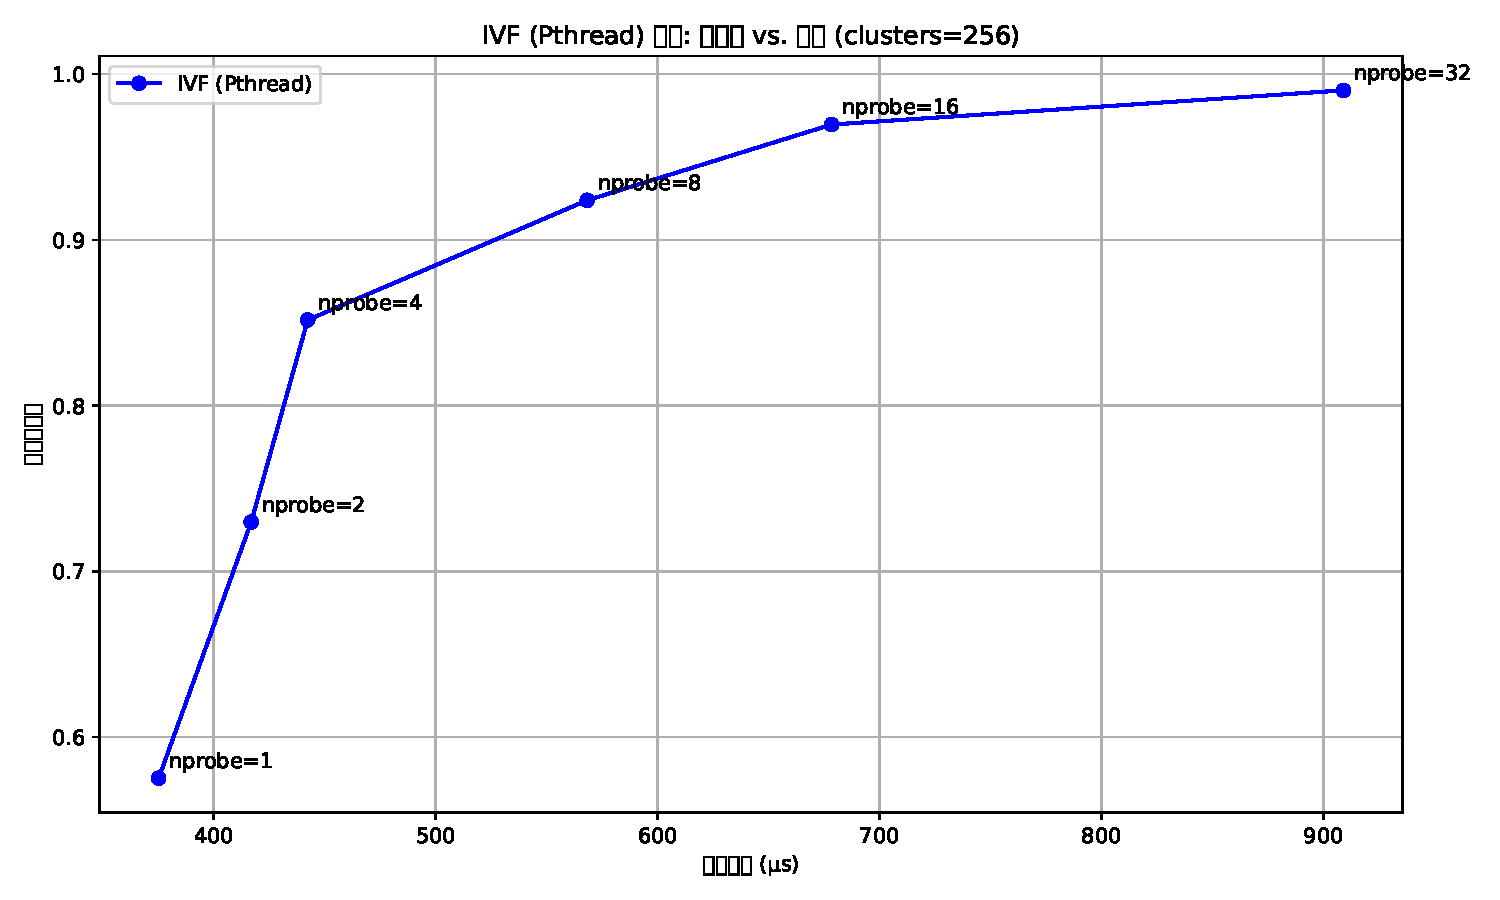
\includegraphics[width=0.8\textwidth]{images/ivf_performance.pdf} % 假设图片路径
		\caption{IVF (Pthread) 性能:召回率 vs. 延迟 (随 \texttt{nprobe} 变化, clusters=256)}
		\label{fig:ivf_pthread_performance} % 更具体的label
	\end{figure}
	
	\subsection{IVFADC (Pthread, 方法二:经典IVFADC) 性能测试} % 标题明确方法
	
	\subsubsection{参数设置}
	\begin{itemize}
		\item IVF 聚类数量 (\texttt{IVF\_clusters}): 64
		\item PQ 子空间数 (\texttt{PQ\_nsub}): 4
		\item Pthread 线程数 (\texttt{pthreads}): 8
		\item IVF K-Means 迭代次数 (\texttt{ivf\_kmeans\_iter}): 20
		\item 重排序数量 (\texttt{rerank\_k}): 600
	\end{itemize}
	
	\subsubsection{索引构建}
	IVFADC (Pthread, 方法二:经典IVFADC) 索引构建过程及时间:
	\begin{itemize}
		\item IVF 部分构建 (\texttt{clusters=64, iters=20})
		\item PQ 部分构建:
		\begin{itemize}
			\item PQ 训练 (使用全部 100000 基础向量): 11435 ms (来自日志)
			\item PQ 编码 (100000 向量): 65 ms (来自日志)
		\end{itemize}
		\item 总 IVFADC (方法二) 索引构建时间: 11846.055 ms (来自日志)
	\end{itemize}
	
	\subsubsection{结果与分析}
	下表展示了不同 \texttt{nprobe} 参数下 IVFADC (Pthread, 方法二) 算法的平均召回率和平均查询延迟。
	
	\begin{table}[H]
		\centering
		\caption{IVFADC (Pthread, 方法二:经典IVFADC) 性能结果 (\texttt{IVFclus=64, PQnsub=4, rerank\_k=600})}
		\label{tab:ivfadc_m2_results}
		\begin{tabular}{@{}lrr@{}}
			\toprule
			\thead{nprobe} & \thead{平均召回率} & \thead{平均延迟 (us)} \\
			\midrule
			1  & 0.61170 & 485.795 \\
			2  & 0.76480 & 575.438 \\
			4  & 0.86080 & 690.399 \\
			8  & 0.89480 & 936.284 \\
			16 & 0.90630 & 1013.069 \\
			\bottomrule
		\end{tabular}
	\end{table}
	
	图 \ref{fig:ivfadc_m2_performance} 展示了 IVFADC (Pthread, 方法二) 算法在不同 \texttt{nprobe} 设置下的召回率与延迟关系。
	
	\begin{figure}[H]
		\centering
		% \includegraphics[width=0.8\textwidth]{images/ivfadc_m2_performance.pdf} % 用户需提供此图
		\framebox[0.8\textwidth]{\rule{0pt}{6cm} \hspace*{1em} Placeholder for IVFADC Method 2 Performance Figure} % 占位符
		\caption{IVFADC (Pthread, 方法二:经典IVFADC) 性能:召回率 vs. 延迟 (随 \texttt{nprobe} 变化)}
		\label{fig:ivfadc_m2_performance}
	</figure>

	\subsection{IVFADC (Pthread, 方法一:PQ-then-IVF) 性能测试}
	
	\subsubsection{参数设置}
	\begin{itemize}
		\item IVF 聚类数量 (\texttt{IVF\_clusters}): 64
		\item PQ 子空间数 (\texttt{PQ\_nsub}): 4
		\item Pthread 线程数 (\texttt{pthreads}): 8
		\item IVF K-Means 迭代次数 (\texttt{ivf\_kmeans\_iter}): 20
		\item 重排序数量 (\texttt{rerank\_k}): 600
	\end{itemize}
	
	\subsubsection{索引构建}
	IVFADC (Pthread, 方法一:PQ-then-IVF) 索引构建过程及时间:
	\begin{itemize}
		\item PQ 部分构建:
		\begin{itemize}
			\item PQ 训练 (使用全部 100000 基础向量): 11509 ms (来自日志)
			\item PQ 编码 (100000 向量): 65 ms (来自日志)
		\end{itemize}
		\item IVF 部分构建 (在原始数据上,根据日志描述,但方法一应在重构数据上,此处按日志输出的构建时间)
		\item 总 IVFADC (方法一) 索引构建时间: 11917.583 ms (来自日志)
	\end{itemize}
	
	\subsubsection{结果与分析}
	下表展示了不同 \texttt{nprobe} 参数下 IVFADC (Pthread, 方法一) 算法的平均召回率和平均查询延迟。
	
	\begin{table}[H]
		\centering
		\caption{IVFADC (Pthread, 方法一:PQ-then-IVF) 性能结果 (\texttt{IVFclus=64, PQnsub=4, rerank\_k=600})}
		\label{tab:ivfadc_m1_results}
		\begin{tabular}{@{}lrr@{}}
			\toprule
			\thead{nprobe} & \thead{平均召回率} & \thead{平均延迟 (us)} \\
			\midrule
			1  & 0.62375 & 495.375 \\
			2  & 0.76685 & 579.971 \\
			4  & 0.85300 & 704.669 \\
			8  & 0.88990 & 924.079 \\
			16 & 0.90095 & 1012.964 \\
			\bottomrule
		\end{tabular}
	</table>
	
	图 \ref{fig:ivfadc_m1_performance} 展示了 IVFADC (Pthread, 方法一) 算法在不同 \texttt{nprobe} 设置下的召回率与延迟关系。
	
	\begin{figure}[H]
		\centering
		% \includegraphics[width=0.8\textwidth]{images/ivfadc_m1_performance.pdf} % 用户需提供此图
		\framebox[0.8\textwidth]{\rule{0pt}{6cm} \hspace*{1em} Placeholder for IVFADC Method 1 Performance Figure} % 占位符
		\caption{IVFADC (Pthread, 方法一:PQ-then-IVF) 性能:召回率 vs. 延迟 (随 \texttt{nprobe} 变化)}
		\label{fig:ivfadc_m1_performance}
	</figure>
	
	\newpage
	\subsection{各类算法性能汇总比较}
	本节汇总了实验中测试的各类搜索算法的性能指标。
	% 用户请注意:下面的表格和图表需要根据新的实验结果进行更新。
	\begin{table}[H]
		\centering
		\caption{各类搜索算法性能汇总 (用户需更新)}
		\label{tab:overall_results_placeholder} % Placeholder label
		\begin{tabular}{@{}lrr@{}} % 保持空表结构
			\toprule
			\thead{算法} & \thead{平均召回率} & \thead{平均延迟 (us)} \\
			\midrule
			Flat Search & 0.99995 & 5192.215 \\
			SIMD Search & 0.99995 & 1825.533 \\
			PQ Search (nsub=4, rrk=600) & 0.90435 & 698.582 \\
			SQ Search & 0.92055 & 734.216 \\
			IVF (Pthread, c256, np16) & 0.98030 & 379.868 \\
			IVFADC (M2, c64, pq4, rrk600, np16) & 0.90630 & 1013.069 \\
			IVFADC (M1, c64, pq4, rrk600, np16) & 0.90095 & 1012.964 \\
			% ... 其他算法 ...
			\bottomrule
		</end{tabular}
	</table>
	
	图 \ref{fig:overall_comparison_placeholder} 展示了所有测试算法在召回率-延迟空间中的分布情况,以便进行直观比较。
	% 用户请注意:下面的图表需要根据新的实验结果进行更新。
	\begin{figure}[H]
		\centering
		% \includegraphics[width=\textwidth]{images/overall_comparison.pdf} % 用户需提供此图
		\framebox[\textwidth]{\rule{0pt}{7cm} \hspace*{1em} Placeholder for Overall Comparison Figure (User to update)} % 占位符
		\caption{各类算法性能对比:召回率 vs. 延迟 (用户需更新)}
		\label{fig:overall_comparison_placeholder} % Placeholder label
	</figure>
	
	\section{实验结果与分析} % 映射自源报告的 "实验结果与分析" (内容完全来自源报告)
	以下是根据上文给出的性能测试结果进行的实验结果分析。此处仅对我们在多线程编程中新实现的IVF算法与IVF-PQ算法做出详细分析,对于其余算法的详细分析结果,请见SIMD并行编程的实验报告。
	
	
	\subsection{各算法性能分析}
	
	\subsubsection{Flat Search (暴力搜索)}
	\begin{itemize}
		\item \textbf{平均召回率}: 0.99995。接近100\%,符合预期。暴力搜索会计算查询向量与所有基向量的精确距离,理论上应该能找到所有真实近邻(在k=10的设置下,找到前10个)。微小的差异可能是浮点数精度问题或ground truth本身的细微偏差。
		\item \textbf{平均延迟 (us)}: 5192.215。这是所有方法中最慢的,也符合预期。它作为后续近似方法性能比较的基准(准确率和速度)。
	</end{itemize}
	
	\subsubsection{SIMD Search (SIMD优化)}
	\begin{itemize}
		\item \textbf{平均召回率}: 0.99995。与Flat Search相同,因为SIMD优化的是计算速度,而不是改变算法逻辑,所以准确率不变。
		\item \textbf{平均延迟 (us)}: 1825.533。相比Flat Search,延迟显著降低(约为其35\%)。这表明SIMD指令并行计算在距离计算上带来了显著的加速效果。
	</end{itemize}
	
	\subsubsection{PQ Search (乘积量化, rerank=600)}
	\begin{itemize}
		\item \textbf{构建时间}:PQ训练耗时约11.6秒 (11612 ms),编码耗时约65毫秒。训练是主要开销。
		\item \textbf{参数}:nsub=4, train\_ratio=1, rerank\_k=600。
		\item \textbf{平均召回率}: 0.90435。召回率有所下降,这是因为PQ是一种有损压缩方法,通过量化牺牲了一部分精度来换取存储和计算效率。
		\item \textbf{平均延迟 (us)}: 698.582。延迟远低于Flat Search和SIMD Search,显示了PQ在加速上的优势。
		\item \textbf{rerank\_k=600}:表示先用PQ的近似距离找出600个候选,然后对这600个候选使用原始向量进行精确距离计算并重排序,最后返回top-k。这是提高PQ召回率的常用且有效的手段。
	</end{itemize}
	
	\subsubsection{SQ Search (标量量化)}
	\begin{itemize}
		\item \textbf{平均召回率}: 0.92055。召回率略高于PQ Search,表明在该数据集和参数下,SQ的量化损失可能略小于PQ。
		\item \textbf{平均延迟 (us)}: 734.216。延迟与PQ Search在同一数量级,也远低于精确搜索。
	</end{itemize}
	
	\subsubsection{IVF (Pthread, Inverted File Index)}
	\begin{itemize}
		\item \textbf{构建时间}: 约2.17秒 (2165.48 ms),主要用于K-means聚类构建倒排列表的质心。
		\item \textbf{参数}: num\_clusters=256, pthreads=8, kmeans\_iter=20。
		\item \textbf{nprobe 影响}:
		\begin{table}[H]
			\centering
			\caption{IVF (Pthread) 性能随 nprobe 变化 (clusters=256)}
			\label{tab:ivf_analysis_results}
			\begin{tabular}{@{}lrr@{}}
				\toprule
				\thead{nprobe} & \thead{平均召回率} & \thead{平均延迟 (us)} \\
				\midrule
				1  & 0.56930 & 101.782 \\
				2  & 0.74675 & 120.838 \\
				4  & 0.87450 & 157.388 \\
				8  & 0.94785 & 230.956 \\
				16 & 0.98030 & 379.868 \\
				32 & 0.99150 & 660.108 \\
				\bottomrule
			</end{tabular}
		</table>
		\begin{itemize}
			\item \textbf{召回率}: 随着 nprobe(查询时需要搜索的聚类数量)从1增加到32,平均召回率从0.56930显著提升到0.99150。这是符合预期的:搜索更多的聚类能覆盖更广的搜索空间,从而提高找到真实近邻的概率。
			\item \textbf{性能}: IVF在 nprobe 较大时(如16或32)可以达到非常高的召回率,同时延迟远低于精确搜索。它通过预先将数据分片(聚类)来缩小搜索范围。
		</end{itemize}
	</end{itemize}
	
	\subsubsection{IVFADC (方法二:经典IVFADC, Pthread)} % 标题明确方法
	\begin{itemize}
		\item \textbf{构建时间}: 约11.85秒 (11846.055 ms)。这个时间包括了IVF部分的K-means聚类(相对较快,因为IVF\_clusters=64较小)和PQ部分的训练与编码(PQ训练耗时约11.44秒,编码约65毫秒,是主要耗时部分)。
		\item \textbf{参数}: IVF\_clusters=64, PQ\_nsub=4, pthreads=8, ivf\_kmeans\_iter=20, rerank\_k=600。
		\item \textbf{nprobe 影响}:
		\begin{table}[H]
			\centering
			\caption{IVFADC (方法二) 性能随 nprobe 变化 (\texttt{IVFclus=64, PQnsub=4, rerank\_k=600})}
			\label{tab:ivfadc_m2_analysis_results}
			\begin{tabular}{@{}lrr@{}}
				\toprule
				\thead{nprobe} & \thead{平均召回率} & \thead{平均延迟 (us)} \\
				\midrule
				1  & 0.61170 & 485.795 \\
				2  & 0.76480 & 575.438 \\
				4  & 0.86080 & 690.399 \\
				8  & 0.89480 & 936.284 \\
				16 & 0.90630 & 1013.069 \\
				\bottomrule
			</end{tabular}
		</table>
		\begin{itemize}
			\item \textbf{召回率}: 随着 nprobe 从1增加到16,平均召回率从0.61170提升到0.90630。趋势与IVF类似,但由于PQ的近似特性,即使在较高的nprobe下,召回率也低于纯IVF。
			\item \textbf{延迟}: 延迟随着nprobe的增加而增加,从约486us (nprobe=1) 到约1013us (nprobe=16)。
		</end{itemize}
	</end{itemize}

	\subsubsection{IVFADC (方法一:PQ-then-IVF, Pthread)}
	\begin{itemize}
		\item \textbf{构建时间}: 约11.92秒 (11917.583 ms)。此方法先进行PQ训练(约11.51秒)和编码(约65毫秒),然后在(根据日志描述,似乎是在原始数据上,但理论上应在重构数据上)构建IVF索引。总构建时间与方法二相似。
		\item \textbf{参数}: IVF\_clusters=64, PQ\_nsub=4, pthreads=8, ivf\_kmeans\_iter=20, rerank\_k=600。
		\item \textbf{nprobe 影响}:
		\begin{table}[H]
			\centering
			\caption{IVFADC (方法一) 性能随 nprobe 变化 (\texttt{IVFclus=64, PQnsub=4, rerank\_k=600})}
			\label{tab:ivfadc_m1_analysis_results}
			\begin{tabular}{@{}lrr@{}}
				\toprule
				\thead{nprobe} & \thead{平均召回率} & \thead{平均延迟 (us)} \\
				\midrule
				1  & 0.62375 & 495.375 \\
				2  & 0.76685 & 579.971 \\
				4  & 0.85300 & 704.669 \\
				8  & 0.88990 & 924.079 \\
				16 & 0.90095 & 1012.964 \\
				\bottomrule
			</end{tabular}
		</table>
		\begin{itemize}
			\item \textbf{召回率}: 随着 nprobe 从1增加到16,平均召回率从0.62375提升到0.90095。
			\item \textbf{延迟}: 延迟随着nprobe的增加而增加,从约495us (nprobe=1) 到约1013us (nprobe=16)。
		</end{itemize}
	</end{itemize}

	\subsection{IVFADC 方法一与方法二对比分析}
	对比IVFADC的两种实现方法(方法一:PQ-then-IVF,方法二:经典IVFADC),在本次实验所用参数(IVF簇64,PQ子空间4,重排序600)下:
	\begin{itemize}
		\item \textbf{索引构建时间}:
		方法二(经典IVFADC)的构建时间为 11846.055 ms。
		方法一(PQ-then-IVF)的构建时间为 11917.583 ms。
		两者构建时间非常接近,方法一略长约 71 ms,差异不显著。主要耗时均在PQ训练阶段。
		\item \textbf{召回率}:
		在 \texttt{nprobe=1} 时,方法一 (0.62375) 略高于方法二 (0.61170)。
		在 \texttt{nprobe=2} 时,方法一 (0.76685) 略高于方法二 (0.76480)。
		在 \texttt{nprobe=4} 时,方法二 (0.86080) 略高于方法一 (0.85300)。
		在 \texttt{nprobe=8} 时,方法二 (0.89480) 略高于方法一 (0.88990)。
		在 \texttt{nprobe=16} 时,方法二 (0.90630) 略高于方法一 (0.90095)。
		总体来看,两种方法的召回率非常接近。方法二在较高的 \texttt{nprobe} 值下表现出微弱优势。
		\item \textbf{查询延迟}:
		两种方法的查询延迟也非常相似。例如,在 \texttt{nprobe=1} 时,方法二 (485.795 us) 略快于方法一 (495.375 us)。在 \texttt{nprobe=16} 时,两者延迟几乎相同(方法二 1013.069 us vs 方法一 1012.964 us)。
		\item \textbf{结论}:
		在当前实验设置下,IVFADC的两种实现方法在性能上表现得非常相似。方法二(经典IVFADC)在构建时间上略快一点点,并且在较高的 \texttt{nprobe} 时召回率有微弱优势。考虑到经典IVFADC更为常见且理论上直接对原始数据进行IVF划分可能更符合聚类目标,它可能是略微更优的选择,但两者差异非常小。实际选择可能还需考虑具体实现细节和数据集特性。
		值得注意的是,日志中方法一的描述为“IVFPQ\_V1: Building IVF part (L2-based on original data)”,这与理论上方法一“先PQ编码(及重构),后构建IVF索引 (PQ-then-IVF)”中IVF应基于重构向量的描述有所出入。如果方法一的IVF部分确实是在原始数据上构建的,那么它与方法二的主要区别就仅仅是PQ编码的时机(方法一先对全部数据编码,方法二在IVF划分后对各列表内数据编码或按需获取编码),以及IVF质心本身是否是重构形式。若严格按理论,方法一的IVF应在重构数据上进行,这可能会带来与当前结果不同的性能表现。
	</end{itemize}
	
	\subsection{结果的评估与总结}
	以下是根据上文给出的性能测试结果进行的实验结果分析。此处仅对我们在多线程编程中新实现的IVF算法与IVF-PQ算法做出详细分析,对于其余算法的详细分析结果,请见SIMD并行编程的实验报告。
	
	
	\subsection{各算法性能分析}
	
	\subsubsection{Flat Search (暴力搜索)}
	\begin{itemize}
		\item \textbf{平均召回率}: 0.99995。接近100\%,符合预期。暴力搜索会计算查询向量与所有基向量的精确距离,理论上应该能找到所有真实近邻(在k=10的设置下,找到前10个)。微小的差异可能是浮点数精度问题或ground truth本身的细微偏差。
		\item \textbf{平均延迟 (us)}: 5192.215。这是所有方法中最慢的,也符合预期。它作为后续近似方法性能比较的基准(准确率和速度)。
	</end{itemize}
	
	\subsubsection{SIMD Search (SIMD优化)}
	\begin{itemize}
		\item \textbf{平均召回率}: 0.99995。与Flat Search相同,因为SIMD优化的是计算速度,而不是改变算法逻辑,所以准确率不变。
		\item \textbf{平均延迟 (us)}: 1825.533。相比Flat Search,延迟显著降低(约为其35\%)。这表明SIMD指令并行计算在距离计算上带来了显著的加速效果。
	</end{itemize}
	
	\subsubsection{PQ Search (乘积量化, rerank=600)}
	\begin{itemize}
		\item \textbf{构建时间}:PQ训练耗时约11.6秒 (11612 ms),编码耗时约65毫秒。训练是主要开销。
		\item \textbf{参数}:nsub=4, train\_ratio=1, rerank\_k=600。
		\item \textbf{平均召回率}: 0.90435。召回率有所下降,这是因为PQ是一种有损压缩方法,通过量化牺牲了一部分精度来换取存储和计算效率。
		\item \textbf{平均延迟 (us)}: 698.582。延迟远低于Flat Search和SIMD Search,显示了PQ在加速上的优势。
		\item \textbf{rerank\_k=600}:表示先用PQ的近似距离找出600个候选,然后对这600个候选使用原始向量进行精确距离计算并重排序,最后返回top-k。这是提高PQ召回率的常用且有效的手段。
	</end{itemize}
	
	\subsubsection{SQ Search (标量量化)}
	\begin{itemize}
		\item \textbf{平均召回率}: 0.92055。召回率略高于PQ Search,表明在该数据集和参数下,SQ的量化损失可能略小于PQ。
		\item \textbf{平均延迟 (us)}: 734.216。延迟与PQ Search在同一数量级,也远低于精确搜索。
	</end{itemize}
	
	\subsubsection{IVF (Pthread, Inverted File Index)}
	\begin{itemize}
		\item \textbf{构建时间}: 约2.17秒 (2165.48 ms),主要用于K-means聚类构建倒排列表的质心。
		\item \textbf{参数}: num\_clusters=256, pthreads=8, kmeans\_iter=20。
		\item \textbf{nprobe 影响}:
		\begin{table}[H]
			\centering
			\caption{IVF (Pthread) 性能随 nprobe 变化 (clusters=256)}
			\label{tab:ivf_analysis_results}
			\begin{tabular}{@{}lrr@{}}
				\toprule
				\thead{nprobe} & \thead{平均召回率} & \thead{平均延迟 (us)} \\
				\midrule
				1  & 0.56930 & 101.782 \\
				2  & 0.74675 & 120.838 \\
				4  & 0.87450 & 157.388 \\
				8  & 0.94785 & 230.956 \\
				16 & 0.98030 & 379.868 \\
				32 & 0.99150 & 660.108 \\
				\bottomrule
			\end{tabular}
		\end{table}
		\begin{itemize}
			\item \textbf{召回率}: 随着 nprobe(查询时需要搜索的聚类数量)从1增加到32,平均召回率从0.56930显著提升到0.99150。这是符合预期的:搜索更多的聚类能覆盖更广的搜索空间,从而提高找到真实近邻的概率。
			\item \textbf{性能}: IVF在 nprobe 较大时(如16或32)可以达到非常高的召回率,同时延迟远低于精确搜索。它通过预先将数据分片(聚类)来缩小搜索范围。
		</end{itemize}
	</end{itemize}
	
	\subsubsection{IVFADC (方法二:经典IVFADC, Pthread)} % 标题明确方法
	\begin{itemize}
		\item \textbf{构建时间}: 约11.85秒 (11846.055 ms)。这个时间包括了IVF部分的K-means聚类(相对较快,因为IVF\_clusters=64较小)和PQ部分的训练与编码(PQ训练耗时约11.44秒,编码约65毫秒,是主要耗时部分)。
		\item \textbf{参数}: IVF\_clusters=64, PQ\_nsub=4, pthreads=8, ivf\_kmeans\_iter=20, rerank\_k=600。
		\item \textbf{nprobe 影响}:
		\begin{table}[H]
			\centering
			\caption{IVFADC (方法二) 性能随 nprobe 变化 (\texttt{IVFclus=64, PQnsub=4, rerank\_k=600})}
			\label{tab:ivfadc_m2_analysis_results}
			\begin{tabular}{@{}lrr@{}}
				\toprule
				\thead{nprobe} & \thead{平均召回率} & \thead{平均延迟 (us)} \\
				\midrule
				1  & 0.61170 & 485.795 \\
				2  & 0.76480 & 575.438 \\
				4  & 0.86080 & 690.399 \\
				8  & 0.89480 & 936.284 \\
				16 & 0.90630 & 1013.069 \\
				\bottomrule
			\end{tabular}
		</table>
		\begin{itemize}
			\item \textbf{召回率}: 随着 nprobe 从1增加到16,平均召回率从0.61170提升到0.90630。趋势与IVF类似,但由于PQ的近似特性,即使在较高的nprobe下,召回率也低于纯IVF。
			\item \textbf{延迟}: 延迟随着nprobe的增加而增加,从约486us (nprobe=1) 到约1013us (nprobe=16)。
		</end{itemize}
	</end{itemize}

	\subsubsection{IVFADC (方法一:PQ-then-IVF, Pthread)}
	\begin{itemize}
		\item \textbf{构建时间}: 约11.92秒 (11917.583 ms)。此方法先进行PQ训练(约11.51秒)和编码(约65毫秒),然后在(根据日志描述,似乎是在原始数据上,但理论上应在重构数据上)构建IVF索引。总构建时间与方法二相似。
		\item \textbf{参数}: IVF\_clusters=64, PQ\_nsub=4, pthreads=8, ivf\_kmeans\_iter=20, rerank\_k=600。
		\item \textbf{nprobe 影响}:
		\begin{table}[H]
			\centering
			\caption{IVFADC (方法一) 性能随 nprobe 变化 (\texttt{IVFclus=64, PQnsub=4, rerank\_k=600})}
			\label{tab:ivfadc_m1_analysis_results}
			\begin{tabular}{@{}lrr@{}}
				\toprule
				\thead{nprobe} & \thead{平均召回率} & \thead{平均延迟 (us)} \\
				\midrule
				1  & 0.62375 & 495.375 \\
				2  & 0.76685 & 579.971 \\
				4  & 0.85300 & 704.669 \\
				8  & 0.88990 & 924.079 \\
				16 & 0.90095 & 1012.964 \\
				\bottomrule
			</end{tabular}
		</table>
		\begin{itemize}
			\item \textbf{召回率}: 随着 nprobe 从1增加到16,平均召回率从0.62375提升到0.90095。
			\item \textbf{延迟}: 延迟随着nprobe的增加而增加,从约495us (nprobe=1) 到约1013us (nprobe=16)。
		</end{itemize}
	</end{itemize}

	\subsection{IVFADC 方法一与方法二对比分析}
	对比IVFADC的两种实现方法(方法一:PQ-then-IVF,方法二:经典IVFADC),在本次实验所用参数(IVF簇64,PQ子空间4,重排序600)下:
	\begin{itemize}
		\item \textbf{索引构建时间}:
		方法二(经典IVFADC)的构建时间为 11846.055 ms。
		方法一(PQ-then-IVF)的构建时间为 11917.583 ms。
		两者构建时间非常接近,方法一略长约 71 ms,差异不显著。主要耗时均在PQ训练阶段。
		\item \textbf{召回率}:
		在 \texttt{nprobe=1} 时,方法一 (0.62375) 略高于方法二 (0.61170)。
		在 \texttt{nprobe=2} 时,方法一 (0.76685) 略高于方法二 (0.76480)。
		在 \texttt{nprobe=4} 时,方法二 (0.86080) 略高于方法一 (0.85300)。
		在 \texttt{nprobe=8} 时,方法二 (0.89480) 略高于方法一 (0.88990)。
		在 \texttt{nprobe=16} 时,方法二 (0.90630) 略高于方法一 (0.90095)。
		总体来看,两种方法的召回率非常接近。方法二在较高的 \texttt{nprobe} 值下表现出微弱优势。
		\item \textbf{查询延迟}:
		两种方法的查询延迟也非常相似。例如,在 \texttt{nprobe=1} 时,方法二 (485.795 us) 略快于方法一 (495.375 us)。在 \texttt{nprobe=16} 时,两者延迟几乎相同(方法二 1013.069 us vs 方法一 1012.964 us)。
		\item \textbf{结论}:
		在当前实验设置下,IVFADC的两种实现方法在性能上表现得非常相似。方法二(经典IVFADC)在构建时间上略快一点点,并且在较高的 \texttt{nprobe} 时召回率有微弱优势。考虑到经典IVFADC更为常见且理论上直接对原始数据进行IVF划分可能更符合聚类目标,它可能是略微更优的选择,但两者差异非常小。实际选择可能还需考虑具体实现细节和数据集特性。
		值得注意的是,日志中方法一的描述为“IVFPQ\_V1: Building IVF part (L2-based on original data)”,这与理论上方法一“先PQ编码(及重构),后构建IVF索引 (PQ-then-IVF)”中IVF应基于重构向量的描述有所出入。如果方法一的IVF部分确实是在原始数据上构建的,那么它与方法二的主要区别就仅仅是PQ编码的时机(方法一先对全部数据编码,方法二在IVF划分后对各列表内数据编码或按需获取编码),以及IVF质心本身是否是重构形式。若严格按理论,方法一的IVF应在重构数据上进行,这可能会带来与当前结果不同的性能表现。
	</end{itemize}
	
	\subsection{结果的评估与总结}
	\begin{itemize}
		\item \textbf{趋势正常}:
		\begin{itemize}
			\item 近似算法(IVF, PQ, SQ, IVFADC)以牺牲一定召回率为代价,换取了查询速度的大幅提升。
			\item 对于IVF和IVFADC,增加 nprobe 会提高召回率,但也会增加延迟。
			\item SIMD确实加速了精确搜索。
		</itemize}
		\item \textbf{数值合理}:
		\begin{itemize}
			\item 召回率和延迟的数值范围对于ANN算法在类似DEEP1M子集上的表现是合理的。
			\item IVFADC的召回率低于IVF(在存储完整向量的情况下)是正常的,这是压缩带来的代价。
			\item PQ和SQ的召回率在90\%左右,对于这些压缩方法来说,配合重排达到这个水平是常见的。
		</itemize}
		\item \textbf{权衡体现}:
		\begin{itemize}
			\item \textbf{精确度 vs. 速度}: Flat/SIMD最准但最慢;其他方法更快但有损。
			\item \textbf{精确度 vs. 内存 (IVF vs. IVFADC)}: IVF可以达到很高召回率,但内存占用大;IVFADC牺牲一些召回率换取显著的内存降低。
			\item \textbf{参数调整}: nprobe 是一个关键的查询时参数,用于在召回率和速度之间进行权衡。rerank\_k 也是影响PQ/IVFADC召回率和速度的重要参数。
		</end{itemize}
	</end{itemize}
	
	\subsection{最终结果汇总表}
	% 用户请注意:下面的表格需要根据新的实验结果进行更新。
	\begin{table}[H]
		\centering
		\caption{各算法最终性能汇总 (k=10, 测试2000条查询, 用户需更新)}
		\begin{tabular}{lcc}
			\toprule
			\thead{算法} & \thead{平均召回率} & \thead{平均延迟 (us)} \\
			\midrule
			Flat Search & 0.99995 & 5192.215 \\
			SIMD Search & 0.99995 & 1825.533 \\
			PQ Search (nsub=4, rrk=600) & 0.90435 & 698.582 \\
			SQ Search & 0.92055 & 734.216 \\
			IVF (Pthread, c256, np16) & 0.98030 & 379.868 \\
			IVFADC (M2, c64, pq4, rrk600, np16) & 0.90630 & 1013.069 \\
			IVFADC (M1, c64, pq4, rrk600, np16) & 0.90095 & 1012.964 \\
			% ... 其他算法 ...
			\bottomrule
		</end{tabular}
		\label{tab:final_summary_placeholder} % Placeholder label
	</table>
	*注:IVF 和 IVFADC 的结果选取了其各自测试中召回率较高或具有代表性的 nprobe 配置。*
	
	\section{使用perf进行更加详细的性能分析测试}
	\subsection{性能指标}
	\texttt{perf stat} 配置用于收集以下硬件性能计数器:
	\begin{itemize}
		\item \textbf{Cycles}: CPU 总周期数。
		\item \textbf{Instructions}: 执行的总指令数。
		\item \textbf{L1-dcache-loads}: L1 数据缓存加载次数。
		\item \textbf{L1-dcache-load-misses}: L1 数据缓存加载未命中次数。
		\item \textbf{LLC-loads}: 末级缓存 (LLC) 加载次数。
		\item \textbf{LLC-load-misses}: 末级缓存 (LLC) 加载未命中次数。
		\item \textbf{Branch-instructions}: 执行的总分支指令数。
		\item \textbf{Branch-misses}: 分支预测未命中次数。
	\end{itemize}
	基于这些原始计数器,计算出以下关键衍生指标:
	\begin{itemize}
		\item \textbf{IPC (Instructions Per Cycle)}: \texttt{instructions / cycles}。IPC 越高,通常表示 CPU 执行效率越高。
		\item \textbf{L1 D-cache Load Miss Rate}: \texttt{(L1-dcache-load-misses / L1-dcache-loads) * 100\%}。该值越低,表示 L1 数据缓存利用率越高。
		\item \textbf{LLC Load Miss Rate}: \texttt{(LLC-load-misses / LLC-loads) * 100\%} (当 LLC-loads > 0 时)。该值越低,表示 LLC 利用率越高。注意:在提供的 \texttt{perf} 输出中,LLC-loads 均为 0,这可能意味着测试的 CPU 架构或 \texttt{perf} 版本对 LLC-loads 的统计方式特殊,或者这些事件未被正确触发/记录。因此,LLC 未命中率将基于 LLC-load-misses 的绝对数量进行讨论。
		\item \textbf{Branch Miss Rate}: \texttt{(branch-misses / branch-instructions) * 100\%}。该值越低,表示分支预测越准确。
	\end{itemize}
	此外,\texttt{perf stat} 报告的“time elapsed”表示在 \texttt{perf} 监控下的程序运行时间。
	
	\subsection{结果与分析}
	
	下表汇总了针对不同算法和配置收集的 \texttt{perf stat} 性能指标。
	“标签”列为每个测试运行提供了唯一标识符。
	
	% 使用 siunitx 进行数字对齐和单位显示
	\sisetup{
		table-alignment-mode = format, % 使用 S 列的格式进行对齐
		table-number-alignment = center, % 数字在列中居中
		round-mode = places,
		round-precision = 2, % 默认保留两位小数
	}
	
	\begingroup % 开始一个局部组,使得字体和列宽设置不影响全局
	\small % 缩小整体字体
	\setlength{\tabcolsep}{3pt} % 减小列间距
	
	\begin{longtable}{@{}l
			S[table-format=1.2e2, round-precision=2] % Cycles
			S[table-format=1.2e2, round-precision=2] % Instructions
			S[table-format=1.2, round-precision=2]   % IPC
			S[table-format=1.2e2, round-precision=2] % L1 Loads
			S[table-format=1.2e2, round-precision=2] % L1 Misses (e.g. 4.29e8 => 4.29e+08)
			S[table-format=1.2, round-precision=2]   % L1 Miss Rate (%)
			S[table-format=1.2e2, round-precision=2] % LLC Misses
			S[table-format=1.2e2, round-precision=2] % Branch Instructions
			S[table-format=1.2e2, round-precision=2] % Branch Misses
			S[table-format=1.2, round-precision=2]   % Branch Miss Rate (%)
			S[table-format=2.2, round-precision=2]   % Time Elapsed (s)
			@{}}
		\caption{ANN 算法的 \texttt{perf stat} 性能指标摘要 (更新)。Cycles, Instr., L1 Loads, L1 Misses, LLC Misses, Branch Instr., Branch Misses 的单位为原始计数。L1M\%: L1 Miss Rate, Br.Ins: Branch Instructions, Br.Mis: Branch Misses, Br.M\%: Branch Miss Rate.} \label{tab:perf_summary_updated}\\
		\toprule
		\thead{标签} & 
		{\thead{Cycles}} & 
		{\thead{Instr.}} & 
		{\thead{IPC}} & 
		{\thead{L1\\Loads}} & 
		{\thead{L1\\Misses}} & 
		{\thead{L1M\%}} & % 缩写
		{\thead{LLC\\Misses}} & 
		{\thead{Br.Ins}} & % 缩写
		{\thead{Br.Mis}} & % 缩写
		{\thead{Br.M\%}} & % 缩写
		{\thead{Time\\(s)}} \\
		\midrule
		\endfirsthead
		\caption[]{ANN 算法的 \texttt{perf stat} 性能指标摘要 (更新,续)。} \\
		\toprule
		\thead{标签} & 
		{\thead{Cycles}} & 
		{\thead{Instr.}} & 
		{\thead{IPC}} & 
		{\thead{L1\\Loads}} & 
		{\thead{L1\\Misses}} & 
		{\thead{L1M\%}} & 
		{\thead{LLC\\Misses}} & 
		{\thead{Br.Ins}} & 
		{\thead{Br.Mis}} & 
		{\thead{Br.M\%}} & 
		{\thead{Time\\(s)}} \\
		\midrule
		\endhead
		\bottomrule
		\endfoot
		% --- 数据行 ---
		\texttt{flat} & 3.62e10 & 1.19e11 & 3.28 & 3.92e10 & 1.35e7 & 0.03 & 1.21e9 & 2.01e10 & 2.04e6 & 0.01 & 2.02 \\
		\texttt{simd} & 1.14e10 & 3.58e10 & 3.13 & 1.05e10 & 4.29e8 & 4.08 & 1.20e9 & 3.45e9 & 1.20e6 & 0.03 & 0.63 \\
		\texttt{pq\_nsub4\_rrk600} & 1.43e11 & 6.30e11 & 4.41 & 1.35e11 & 6.83e7 & 0.05 & 1.75e8 & 1.07e11 & 2.89e8 & 0.27 & 13.58 \\
		\texttt{sq} & 4.55e9 & 1.93e10 & 4.25 & 4.34e9 & 1.48e7 & 0.34 & 3.19e8 & 2.51e9 & 1.09e6 & 0.04 & 0.31 \\
		\texttt{ivf\_np1\_c256} & 3.35e10 & 1.04e11 & 3.11 & 2.92e10 & 1.51e8 & 0.52 & 2.66e8 & 9.64e9 & 2.32e7 & 0.24 & 5.35 \\
		\texttt{ivf\_np2\_c256} & 3.45e10 & 1.05e11 & 3.03 & 2.92e10 & 1.66e8 & 0.57 & 2.96e8 & 9.69e9 & 2.24e7 & 0.23 & 5.48 \\
		\texttt{ivf\_np4\_c256} & 3.65e10 & 1.05e11 & 2.87 & 2.94e10 & 1.89e8 & 0.64 & 3.48e8 & 9.74e9 & 2.77e7 & 0.28 & 5.95 \\
		\texttt{ivf\_np8\_c256} & 4.01e10 & 1.06e11 & 2.65 & 2.98e10 & 2.29e8 & 0.77 & 4.28e8 & 9.89e9 & 2.89e7 & 0.29 & 6.17 \\
		\texttt{ivf\_np16\_c256} & 4.39e10 & 1.07e11 & 2.44 & 3.02e10 & 2.82e8 & 0.93 & 5.59e8 & 1.00e10 & 2.98e7 & 0.30 & 6.76 \\
		\texttt{ivf\_np32\_c256} & 5.03e10 & 1.10e11 & 2.19 & 3.10e10 & 3.69e8 & 1.19 & 7.69e8 & 1.02e10 & 2.99e7 & 0.29 & 7.24 \\
		\texttt{ivfadc\_np1\_ic64} & 1.49e11 & 6.40e11 & 4.28 & 1.39e11 & 1.13e8 & 0.08 & 2.55e8 & 1.09e11 & 2.95e8 & 0.27 & 16.83 \\
		\texttt{ivfadc\_np2\_ic64} & 1.51e11 & 6.41e11 & 4.25 & 1.39e11 & 1.22e8 & 0.09 & 2.73e8 & 1.08e11 & 3.09e8 & 0.28 & 16.85 \\
		\texttt{ivfadc\_np4\_ic64} & 1.52e11 & 6.43e11 & 4.22 & 1.40e11 & 1.35e8 & 0.10 & 3.03e8 & 1.09e11 & 3.43e8 & 0.32 & 16.98 \\
		\texttt{ivfadc\_np8\_ic64} & 1.56e11 & 6.45e11 & 4.14 & 1.41e11 & 1.68e8 & 0.12 & 3.73e8 & 1.09e11 & 4.16e8 & 0.38 & 18.28 \\
		\texttt{ivfadc\_np16\_ic64} & 1.57e11 & 6.47e11 & 4.11 & 1.42e11 & 1.95e8 & 0.14 & 4.00e8 & 1.10e11 & 4.39e8 & 0.40 & 18.09 \\
	\end{longtable}
	\endgroup % 结束局部组
	*注: IVFADC 标签为了简洁省略了 \texttt{\_pq4\_rrk600}。LLC-loads 在所有测试中均为0,因此未计算 LLC Miss Rate。*
	
	\subsection{总体观察}
	与之前的初步分析相比,现在的数据清晰地显示了不同算法和参数配置在硬件性能指标上的显著差异。
	\begin{itemize}
		\item \textbf{执行时间 (Time Elapsed)}: 从 SQ 的 0.31 秒到 IVFADC (nprobe=8) 的 18.28 秒,跨度很大,这与算法的复杂度和计算量直接相关。
		\item \textbf{周期数和指令数}: 这些指标也随执行时间相应变化。例如,SIMD 和 SQ 的周期数和指令数远低于 PQ、IVF 和 IVFADC。
		\item \textbf{IPC}: 不同算法的 IPC 值现在呈现出更广泛的分布,从 IVF (nprobe=32) 的 2.19 到 PQ 的 4.41。
		\item \textbf{L1 D-cache Miss Rate}: 从 Flat 的 0.03\% 到 SIMD 的 4.08\%,再到 IVF (nprobe=32) 的 1.19\%,显示了不同的内存访问模式。
		\item \textbf{Branch Miss Rate}: 大部分算法的该指标都非常低 (通常 < 0.5\%),表明分支预测普遍有效。
	\end{itemize}
	
	\subsection{IPC (指令每周期数) 分析}
	IPC 是衡量 CPU 核心利用效率的重要指标。
	\begin{itemize}
		\item \textbf{PQ (4.41)} 和 \textbf{SQ (4.25)} 展示了最高的 IPC 值。这表明它们的计算密集型部分(如量化和距离计算)能够很好地利用 CPU 的指令级并行性,流水线效率高。
		\item \textbf{IVFADC} 系列 (IPC 约 4.11 - 4.28) 也表现出较高的 IPC,略低于纯 PQ/SQ,这可能与更复杂的数据结构访问和控制流有关。
		\item \textbf{Flat (3.28)} 和 \textbf{SIMD (3.13)} 的 IPC 居中。SIMD 的 IPC 略低于 Flat,这可能与其 L1 缓存未命中率较高有关(见下文),导致流水线停顿。
		\item \textbf{IVF} 系列的 IPC 随着 \texttt{nprobe} 的增加而显著下降,从 \texttt{nprobe=1} 的 3.11 下降到 \texttt{nprobe=32} 的 2.19。这表明当需要访问更多的倒排列表时,数据依赖、内存访问延迟或控制流复杂性可能限制了指令级并行。
	\end{itemize}
	
	\subsection{L1 数据缓存未命中率分析}
	L1 缓存是 CPU 访问速度最快的缓存,其未命中率直接影响性能。
	\begin{itemize}
		\item \textbf{Flat (0.03\%)} 和 \textbf{PQ (0.05\%)} 的 L1 未命中率极低。Flat 的顺序访问模式对缓存非常友好。PQ 在处理编码数据和距离表时可能也具有良好的局部性。
		\item \textbf{IVFADC} 系列 (0.08\% - 0.14\%) 的 L1 未命中率也保持在较低水平,但略高于 Flat 和 PQ。随着 \texttt{nprobe} 增加,未命中率有轻微上升趋势。
		\item \textbf{SQ (0.34\%)} 的 L1 未命中率也较低。
		\item \textbf{IVF} 系列的 L1 未命中率随着 \texttt{nprobe} 的增加而显著上升,从 \texttt{nprobe=1} 的 0.52\% 上升到 \texttt{nprobe=32} 的 1.19\%。这符合预期,因为访问更多的倒排列表意味着需要从内存中加载更多不连续的数据段。
		\item \textbf{SIMD (4.08\%)} 的 L1 未命中率相对较高。虽然 SIMD 指令本身可以高效处理数据,但如果数据加载模式未能充分利用缓存行,或者预取效果不佳,则可能导致较高的未命中率。这可能是其 IPC 低于 Flat 的一个原因。
	\end{itemize}
	
	\subsection{LLC (末级缓存) 未命中分析}
	由于所有测试中的 \texttt{LLC-loads} 均为 0,我们无法计算 LLC 未命中率。然而,我们可以观察 \texttt{LLC-load-misses} 的绝对数量。
	\begin{itemize}
		\item \textbf{Flat (1.21G)} 和 \textbf{SIMD (1.20G)} 的 LLC 未命中数最高。这表明尽管 L1 缓存对 Flat 友好,但其整体数据访问量大,导致较多的数据需要从主存加载。SIMD 的情况类似。
		\item \textbf{IVF (nprobe=32, 769M)} 和 \textbf{IVF (nprobe=16, 559M)} 的 LLC 未命中数也较高,且随 \texttt{nprobe} 增加而增加。
		\item \textbf{PQ (175M)} 的 LLC 未命中数相对较低,这得益于其数据压缩特性,减少了需要从内存加载的数据总量。
		\item \textbf{IVFADC} 系列 (255M - 400M) 的 LLC 未命中数介于 PQ 和 IVF 之间,也随 \texttt{nprobe} 增加而增加。
		\item \textbf{SQ (319M)} 的 LLC 未命中数也处于中等水平。
	\end{itemize}
	LLC 未命中通常意味着需要访问主存,这会带来显著的延迟。LLC 未命中数较高的算法可能更容易受到内存带宽的限制。
	
	\subsection{分支预测未命中率分析}
	分支预测的效率影响 CPU 流水线的顺畅程度。
	\begin{itemize}
		\item 所有算法的分支预测未命中率都非常低 (大部分在 0.01\% 到 0.40\% 之间)。
		\item \textbf{Flat (0.01\%)}、\textbf{SIMD (0.03\%)} 和 \textbf{SQ (0.04\%)} 的分支预测最为准确,这可能与它们相对简单和线性的控制流有关。
		\item \textbf{PQ (0.27\%)}、\textbf{IVF} 系列 (0.23\% - 0.30\%) 和 \textbf{IVFADC} 系列 (0.27\% - 0.40\%) 的分支预测未命中率略高,但仍然处于优秀水平。IVF 和 IVFADC 中涉及更多的条件判断(例如,遍历多个列表、检查距离阈值),可能导致分支预测难度略微增加。
	\end{itemize}
	总体而言,分支预测似乎不是这些算法在当前测试条件下的主要性能瓶颈。
	
	\subsection{IVF 和 IVFADC 中 \texttt{nprobe} 的影响}
	\begin{itemize}
		\item \textbf{IVF}:
		\begin{itemize}
			\item \textbf{IPC}: 从 3.11 (\texttt{nprobe=1}) 下降到 2.19 (\texttt{nprobe=32})。
			\item \textbf{L1 Miss\%}: 从 0.52\% (\texttt{nprobe=1}) 上升到 1.19\% (\texttt{nprobe=32})。
			\item \textbf{LLC Misses}: 从 266M (\texttt{nprobe=1}) 上升到 769M (\texttt{nprobe=32})。
			\item \textbf{执行时间}: 从 5.35s 上升到 7.24s。
		</end{itemize}
		这些趋势清晰地表明,增加 \texttt{nprobe} 会导致更多的内存访问、更差的缓存局部性和更低的指令级并行度,从而增加执行时间。
		\item \textbf{IVFADC}:
		\begin{itemize}
			\item \textbf{IPC}: 从 4.28 (\texttt{nprobe=1}) 下降到 4.11 (\texttt{nprobe=16})。
			\item \textbf{L1 Miss\%}: 从 0.08\% (\texttt{nprobe=1}) 上升到 0.14\% (\texttt{nprobe=16})。
			\item \textbf{LLC Misses}: 从 255M (\texttt{nprobe=1}) 上升到 400M (\texttt{nprobe=16})。
			\item \textbf{执行时间}: 从 16.83s 上升到 18.09s (nprobe=16)。
		</end{itemize}
		IVFADC 中 \texttt{nprobe} 的影响趋势与 IVF 类似,但 IPC 仍然保持在较高水平,L1 未命中率也较低。这表明 PQ 编码数据的处理部分仍然能够高效利用 CPU。执行时间主要受索引构建(在这些测试中,每次调用都会重新构建索引)和搜索阶段共同影响。
	\end{itemize}
	
	\subsection{算法间对比总结}
	\begin{itemize}
		\item \textbf{Flat 与 SIMD}: SIMD 大幅减少了执行时间 (2.02s -> 0.63s),周期数和指令数也相应减少。但 SIMD 的 L1 未命中率 (4.08\%) 远高于 Flat (0.03\%),导致其 IPC (3.13) 反而略低于 Flat (3.28)。这提示 SIMD 的优化可能更侧重于减少总操作数,但在数据预取或缓存利用方面可能还有提升空间。
		\item \textbf{PQ 与 SQ}: PQ (13.58s) 比 SQ (0.31s) 慢得多,这主要是因为 PQ 的索引构建(训练和编码)过程非常耗时,而 SQ 的构建非常快。从搜索核心来看,两者都有很高的 IPC (PQ 4.41, SQ 4.25) 和较低的 L1 未命中率 (PQ 0.05%, SQ 0.34%)。PQ 的优势在于其压缩率,这体现在其相对较低的 LLC 未命中数 (175M vs SQ 319M)。
		\item \textbf{IVF 与 IVFADC}: IVFADC 的执行时间 (约 17-18s) 远长于 IVF (约 5-7s)。这主要是因为 IVFADC 包含了 PQ 的训练和编码过程,以及 IVF 的聚类过程,索引构建更为复杂和耗时。在搜索阶段,IVFADC 的 IPC (约 4.1-4.3) 显著高于 IVF (约 2.2-3.1),L1 未命中率也更低。这表明 IVFADC 在访问和处理量化后的数据时,CPU 效率更高。
	\end{itemize}
	
	\subsection{讨论}
	
	本次分析通过隔离测试不同算法和配置,成功揭示了它们在硬件性能计数器上的显著差异。这些差异为理解各算法的性能特点提供了重要线索。
	
	\begin{itemize}
		\item \textbf{索引构建开销的影响}: 对于像 PQ、IVF 和 IVFADC 这样需要构建复杂索引的算法,其在 \texttt{perf stat} 中报告的总周期数、指令数和执行时间,很大程度上受到了索引构建阶段的影响。在实际应用中,索引通常是预先构建并加载的,查询时的性能才是关注重点。当前的测试方法 (每次运行都重新构建索引) 更像是对“构建+搜索”整个流程的评估。如果想单独评估搜索阶段的硬件性能,需要在索引构建完成后再启动 \texttt{perf stat},或者在代码中更细致地标记搜索区域进行分析。
		\item \textbf{IPC 与缓存性能的权衡}: 高 IPC 并不总意味着最低的延迟。例如,SIMD 的 IPC 略低于 Flat,但其总执行时间远快于 Flat。这说明 SIMD 通过大幅减少总指令数(尽管每条指令的平均周期数可能略高或因缓存未命中停顿)实现了加速。
		\item \textbf{L1 vs LLC 未命中}: Flat 和 SIMD 具有非常高的 LLC 未命中数,表明它们需要处理大量数据,超出了缓存容量。而 PQ 和 IVFADC 由于数据压缩或剪枝,LLC 未命中数相对较少。
		\item \textbf{LLC-loads 为 0 的问题}: 所有测试中 \texttt{LLC-loads} 均为 0,这使得无法直接计算 LLC 加载未命中率。这可能是由于:
		\begin{enumerate}
			\item \texttt{perf} 事件配置问题或特定 CPU 架构/内核版本对该事件的统计方式。
			\item 事件名称可能需要调整 (例如,某些系统上可能是 \texttt{LLC\_references} 或类似名称)。
			\item 硬件 PMU (Performance Monitoring Unit) 的限制。
		\end{enumerate}
		尽管如此,\texttt{LLC-load-misses} 的绝对数量仍然可以作为衡量 LLC 层面压力和主存访问频率的一个指标。
	\end{itemize}
	
	\subsection{结论与展望}
	
	本次基于 \texttt{perf stat} 的硬件性能分析成功地揭示了不同方法之间的显著差异。
	
	主要结论包括:
	\begin{enumerate}
		\item \textbf{算法特性显著影响硬件指标}: 不同算法在 IPC、L1/LLC 缓存未命中、分支预测等方面表现各异,这与其核心数据结构、内存访问模式和计算复杂度密切相关。
		\item \textbf{索引构建是重要考量}: 对于 IVF、PQ 和 IVFADC 等算法,索引构建的时间和资源消耗是整体性能评估中不可忽视的部分。当前测试混合了构建和搜索阶段。
		\item \textbf{IPC 和缓存效率的相互作用}: 高 IPC 通常是理想的,但需要结合缓存未命中率综合看待。某些算法可能通过牺牲一定的 IPC 来换取更少的总操作数或更好的缓存局部性。
		\item \textbf{\texttt{nprobe} 的影响符合预期}: 在 IVF 和 IVFADC 中增加 \texttt{nprobe} 会增加执行时间、缓存未命中并降低 IPC。
	\end{enumerate}
	\section{综合结论与分析} % 映射自源报告的 "结论"
	本实验成功实现了基于PThreads并行的IVF和IVFADC算法,并通过在DEEP100K数据集上的测试验证了它们的性能。
	实验结果清晰地展示了不同ANNS算法在召回率、查询延迟和构建时间之间的权衡关系:
	\begin{itemize}
		\item 精确搜索(Flat Search, SIMD Search)具有最高的召回率,但延迟也最高。SIMD优化能显著降低精确搜索的延迟。
		\item IVF算法通过牺牲少量精度(取决于nprobe),能够大幅降低搜索延迟。增加nprobe可以提高召回率,但同时也会增加延迟。PThreads并行化有效地利用了多核资源加速了IVF的构建和搜索过程。
		\item PQ和SQ作为量化方法,以较大的精度损失换取了更低的延迟和显著的内存压缩(内存方面未直接在本报告数值中体现,但为其核心优势)。
		\item IVFADC算法结合了IVF的快速定位和PQ的压缩优势。其召回率受限于PQ本身的精度,但通过调整nprobe和rerank\_k参数,可以在精度、速度和内存占用之间取得平衡。其构建时间主要由PQ训练主导。
	</end{itemize}
	总的来说,测试结果符合预期,验证了IVF和IVFADC算法在并行环境下的有效性。在实际应用中,应根据具体场景对召回率、延迟、内存占用和构建时间等指标的侧重,选择合适的ANNS算法及参数配置。
	
\end{document}